\documentclass[twoside]{book}

% Packages required by doxygen
\usepackage{fixltx2e}
\usepackage{calc}
\usepackage{doxygen}
\usepackage[export]{adjustbox} % also loads graphicx
\usepackage{graphicx}
\usepackage[utf8]{inputenc}
\usepackage{makeidx}
\usepackage{multicol}
\usepackage{multirow}
\PassOptionsToPackage{warn}{textcomp}
\usepackage{textcomp}
\usepackage[nointegrals]{wasysym}
\usepackage[table]{xcolor}

% Font selection
\usepackage[T1]{fontenc}
\usepackage[scaled=.90]{helvet}
\usepackage{courier}
\usepackage{amssymb}
\usepackage{sectsty}
\renewcommand{\familydefault}{\sfdefault}
\allsectionsfont{%
  \fontseries{bc}\selectfont%
  \color{darkgray}%
}
\renewcommand{\DoxyLabelFont}{%
  \fontseries{bc}\selectfont%
  \color{darkgray}%
}
\newcommand{\+}{\discretionary{\mbox{\scriptsize$\hookleftarrow$}}{}{}}

% Page & text layout
\usepackage{geometry}
\geometry{%
  a4paper,%
  top=2.5cm,%
  bottom=2.5cm,%
  left=2.5cm,%
  right=2.5cm%
}
\tolerance=750
\hfuzz=15pt
\hbadness=750
\setlength{\emergencystretch}{15pt}
\setlength{\parindent}{0cm}
\setlength{\parskip}{3ex plus 2ex minus 2ex}
\makeatletter
\renewcommand{\paragraph}{%
  \@startsection{paragraph}{4}{0ex}{-1.0ex}{1.0ex}{%
    \normalfont\normalsize\bfseries\SS@parafont%
  }%
}
\renewcommand{\subparagraph}{%
  \@startsection{subparagraph}{5}{0ex}{-1.0ex}{1.0ex}{%
    \normalfont\normalsize\bfseries\SS@subparafont%
  }%
}
\makeatother

% Headers & footers
\usepackage{fancyhdr}
\pagestyle{fancyplain}
\fancyhead[LE]{\fancyplain{}{\bfseries\thepage}}
\fancyhead[CE]{\fancyplain{}{}}
\fancyhead[RE]{\fancyplain{}{\bfseries\leftmark}}
\fancyhead[LO]{\fancyplain{}{\bfseries\rightmark}}
\fancyhead[CO]{\fancyplain{}{}}
\fancyhead[RO]{\fancyplain{}{\bfseries\thepage}}
\fancyfoot[LE]{\fancyplain{}{}}
\fancyfoot[CE]{\fancyplain{}{}}
\fancyfoot[RE]{\fancyplain{}{\bfseries\scriptsize Generated by Doxygen }}
\fancyfoot[LO]{\fancyplain{}{\bfseries\scriptsize Generated by Doxygen }}
\fancyfoot[CO]{\fancyplain{}{}}
\fancyfoot[RO]{\fancyplain{}{}}
\renewcommand{\footrulewidth}{0.4pt}
\renewcommand{\chaptermark}[1]{%
  \markboth{#1}{}%
}
\renewcommand{\sectionmark}[1]{%
  \markright{\thesection\ #1}%
}

% Indices & bibliography
\usepackage{natbib}
\usepackage[titles]{tocloft}
\setcounter{tocdepth}{3}
\setcounter{secnumdepth}{5}
\makeindex

% Hyperlinks (required, but should be loaded last)
\usepackage{ifpdf}
\ifpdf
  \usepackage[pdftex,pagebackref=true]{hyperref}
\else
  \usepackage[ps2pdf,pagebackref=true]{hyperref}
\fi
\hypersetup{%
  colorlinks=true,%
  linkcolor=blue,%
  citecolor=blue,%
  unicode%
}

% Custom commands
\newcommand{\clearemptydoublepage}{%
  \newpage{\pagestyle{empty}\cleardoublepage}%
}

\usepackage{caption}
\captionsetup{labelsep=space,justification=centering,font={bf},singlelinecheck=off,skip=4pt,position=top}

%===== C O N T E N T S =====

\begin{document}

% Titlepage & ToC
\hypersetup{pageanchor=false,
             bookmarksnumbered=true,
             pdfencoding=unicode
            }
\pagenumbering{alph}
\begin{titlepage}
\vspace*{7cm}
\begin{center}%
{\Large P\+PL Project }\\
\vspace*{1cm}
{\large Generated by Doxygen 1.8.13}\\
\end{center}
\end{titlepage}
\clearemptydoublepage
\pagenumbering{roman}
\tableofcontents
\clearemptydoublepage
\pagenumbering{arabic}
\hypersetup{pageanchor=true}

%--- Begin generated contents ---
\chapter{P\+P\+L-\/\+Assignment}
\label{md___users_invokesus_assignment__r_e_a_d_m_e}
\Hypertarget{md___users_invokesus_assignment__r_e_a_d_m_e}
\paragraph*{Souvik Sen -\/ I\+I\+T2015505}

{\bfseries To generate new testing data}


\begin{DoxyCode}
python3 tester.py
\end{DoxyCode}


{\bfseries To form Couples from the generated test data}


\begin{DoxyCode}
python3 q1.py
\end{DoxyCode}


{\bfseries To perform gifting and to find the happiest and most compatible k couples}


\begin{DoxyCode}
python3 q2.py
\end{DoxyCode}


{\bfseries To view the logs}


\begin{DoxyCode}
cat logs.txt
\end{DoxyCode}


{\bfseries To view docs}


\begin{DoxyCode}
bash ./doc.sh
\end{DoxyCode}
 Or open ./docs/html/index.html in your browser to view it directly. 
\chapter{Namespace Index}
\section{Packages}
Here are the packages with brief descriptions (if available)\+:\begin{DoxyCompactList}
\item\contentsline{section}{\hyperlink{namespaceq2__helper}{q2\+\_\+helper} }{\pageref{namespaceq2__helper}}{}
\end{DoxyCompactList}

\chapter{Hierarchical Index}
\section{Class Hierarchy}
This inheritance list is sorted roughly, but not completely, alphabetically\+:\begin{DoxyCompactList}
\item object\begin{DoxyCompactList}
\item \contentsline{section}{boy.\+Boy}{\pageref{classboy_1_1_boy}}{}
\begin{DoxyCompactList}
\item \contentsline{section}{geek\+\_\+boy.\+Geek\+\_\+\+Boy}{\pageref{classgeek__boy_1_1_geek___boy}}{}
\item \contentsline{section}{generous\+\_\+boy.\+Generous\+\_\+\+Boy}{\pageref{classgenerous__boy_1_1_generous___boy}}{}
\item \contentsline{section}{miser\+\_\+boy.\+Miser\+\_\+\+Boy}{\pageref{classmiser__boy_1_1_miser___boy}}{}
\end{DoxyCompactList}
\item \contentsline{section}{couple.\+Couple}{\pageref{classcouple_1_1_couple}}{}
\item \contentsline{section}{gift.\+Gift}{\pageref{classgift_1_1_gift}}{}
\begin{DoxyCompactList}
\item \contentsline{section}{essential\+\_\+gift.\+Essential\+\_\+\+Gift}{\pageref{classessential__gift_1_1_essential___gift}}{}
\item \contentsline{section}{luxury\+\_\+gift.\+Luxury\+\_\+\+Gift}{\pageref{classluxury__gift_1_1_luxury___gift}}{}
\item \contentsline{section}{utility\+\_\+gift.\+Utility\+\_\+\+Gift}{\pageref{classutility__gift_1_1_utility___gift}}{}
\end{DoxyCompactList}
\item \contentsline{section}{girl.\+Girl}{\pageref{classgirl_1_1_girl}}{}
\begin{DoxyCompactList}
\item \contentsline{section}{choosy\+\_\+girl.\+Choosy\+\_\+\+Girl}{\pageref{classchoosy__girl_1_1_choosy___girl}}{}
\item \contentsline{section}{desperate\+\_\+girl.\+Desperate\+\_\+\+Girl}{\pageref{classdesperate__girl_1_1_desperate___girl}}{}
\item \contentsline{section}{normal\+\_\+girl.\+Normal\+\_\+\+Girl}{\pageref{classnormal__girl_1_1_normal___girl}}{}
\end{DoxyCompactList}
\end{DoxyCompactList}
\end{DoxyCompactList}

\chapter{Class Index}
\section{Class List}
Here are the classes, structs, unions and interfaces with brief descriptions\+:\begin{DoxyCompactList}
\item\contentsline{section}{\hyperlink{classboy_1_1_boy}{boy.\+Boy} }{\pageref{classboy_1_1_boy}}{}
\item\contentsline{section}{\hyperlink{classchoosy__girl_1_1_choosy___girl}{choosy\+\_\+girl.\+Choosy\+\_\+\+Girl} }{\pageref{classchoosy__girl_1_1_choosy___girl}}{}
\item\contentsline{section}{\hyperlink{classcouple_1_1_couple}{couple.\+Couple} }{\pageref{classcouple_1_1_couple}}{}
\item\contentsline{section}{\hyperlink{classdesperate__girl_1_1_desperate___girl}{desperate\+\_\+girl.\+Desperate\+\_\+\+Girl} }{\pageref{classdesperate__girl_1_1_desperate___girl}}{}
\item\contentsline{section}{\hyperlink{classessential__gift_1_1_essential___gift}{essential\+\_\+gift.\+Essential\+\_\+\+Gift} }{\pageref{classessential__gift_1_1_essential___gift}}{}
\item\contentsline{section}{\hyperlink{classgeek__boy_1_1_geek___boy}{geek\+\_\+boy.\+Geek\+\_\+\+Boy} }{\pageref{classgeek__boy_1_1_geek___boy}}{}
\item\contentsline{section}{\hyperlink{classgenerous__boy_1_1_generous___boy}{generous\+\_\+boy.\+Generous\+\_\+\+Boy} }{\pageref{classgenerous__boy_1_1_generous___boy}}{}
\item\contentsline{section}{\hyperlink{classgift_1_1_gift}{gift.\+Gift} }{\pageref{classgift_1_1_gift}}{}
\item\contentsline{section}{\hyperlink{classgirl_1_1_girl}{girl.\+Girl} }{\pageref{classgirl_1_1_girl}}{}
\item\contentsline{section}{\hyperlink{classluxury__gift_1_1_luxury___gift}{luxury\+\_\+gift.\+Luxury\+\_\+\+Gift} }{\pageref{classluxury__gift_1_1_luxury___gift}}{}
\item\contentsline{section}{\hyperlink{classmiser__boy_1_1_miser___boy}{miser\+\_\+boy.\+Miser\+\_\+\+Boy} }{\pageref{classmiser__boy_1_1_miser___boy}}{}
\item\contentsline{section}{\hyperlink{classnormal__girl_1_1_normal___girl}{normal\+\_\+girl.\+Normal\+\_\+\+Girl} }{\pageref{classnormal__girl_1_1_normal___girl}}{}
\item\contentsline{section}{\hyperlink{classutility__gift_1_1_utility___gift}{utility\+\_\+gift.\+Utility\+\_\+\+Gift} }{\pageref{classutility__gift_1_1_utility___gift}}{}
\end{DoxyCompactList}

\chapter{Namespace Documentation}
\hypertarget{namespaceq2__helper}{}\section{q2\+\_\+helper Namespace Reference}
\label{namespaceq2__helper}\index{q2\+\_\+helper@{q2\+\_\+helper}}
\subsection*{Functions}
\begin{DoxyCompactItemize}
\item 
def \hyperlink{namespaceq2__helper_a8b3d3b435300fd1f72d5dcf384d378ae}{gift\+\_\+sort} ()
\item 
def \hyperlink{namespaceq2__helper_ac0013034c33667bd83f64de880d2d177}{gifting} (couples\+\_\+list, gift\+\_\+list)
\item 
\mbox{\Hypertarget{namespaceq2__helper_aa1be2d7c40a76485c6c99c01d70f7f94}\label{namespaceq2__helper_aa1be2d7c40a76485c6c99c01d70f7f94}} 
def {\bfseries sort\+\_\+by\+\_\+happiness} (couples\+\_\+list)
\item 
\mbox{\Hypertarget{namespaceq2__helper_ac8e0cbab1bea854b3f1457f81b26324f}\label{namespaceq2__helper_ac8e0cbab1bea854b3f1457f81b26324f}} 
def {\bfseries sort\+\_\+by\+\_\+compatibility} (couples\+\_\+list)
\end{DoxyCompactItemize}
\subsection*{Variables}
\begin{DoxyCompactItemize}
\item 
\mbox{\Hypertarget{namespaceq2__helper_a707dcdaaab43b6d4969a0cb3cabe7f8d}\label{namespaceq2__helper_a707dcdaaab43b6d4969a0cb3cabe7f8d}} 
int {\bfseries k} = 1
\item 
\mbox{\Hypertarget{namespaceq2__helper_a17733fc799bfce7e94f29dc9f8d0538e}\label{namespaceq2__helper_a17733fc799bfce7e94f29dc9f8d0538e}} 
{\bfseries format}
\item 
\mbox{\Hypertarget{namespaceq2__helper_ae8d3b2c21f94189201a72219b15efff5}\label{namespaceq2__helper_ae8d3b2c21f94189201a72219b15efff5}} 
{\bfseries datefmt}
\item 
\mbox{\Hypertarget{namespaceq2__helper_a6bf9379ce8dbb3cbe4e6cce5844d5be2}\label{namespaceq2__helper_a6bf9379ce8dbb3cbe4e6cce5844d5be2}} 
{\bfseries level}
\item 
\mbox{\Hypertarget{namespaceq2__helper_a3ff914f74a8a008805e4f07bda9723d6}\label{namespaceq2__helper_a3ff914f74a8a008805e4f07bda9723d6}} 
{\bfseries D\+E\+B\+UG}
\item 
\mbox{\Hypertarget{namespaceq2__helper_a576aee952f4e47794fcdb43c4aebeb49}\label{namespaceq2__helper_a576aee952f4e47794fcdb43c4aebeb49}} 
{\bfseries filename}
\item 
\mbox{\Hypertarget{namespaceq2__helper_a7d612174511c4ec56695533c317cfdc6}\label{namespaceq2__helper_a7d612174511c4ec56695533c317cfdc6}} 
{\bfseries filemode}
\end{DoxyCompactItemize}


\subsection{Detailed Description}
\begin{DoxyVerb}Helper module for q2.py
Has functions to perform sorting of gifts, gifting, sorting of couples according to happiness and compatibility\end{DoxyVerb}
 

\subsection{Function Documentation}
\mbox{\Hypertarget{namespaceq2__helper_a8b3d3b435300fd1f72d5dcf384d378ae}\label{namespaceq2__helper_a8b3d3b435300fd1f72d5dcf384d378ae}} 
\index{q2\+\_\+helper@{q2\+\_\+helper}!gift\+\_\+sort@{gift\+\_\+sort}}
\index{gift\+\_\+sort@{gift\+\_\+sort}!q2\+\_\+helper@{q2\+\_\+helper}}
\subsubsection{\texorpdfstring{gift\+\_\+sort()}{gift\_sort()}}
{\footnotesize\ttfamily def q2\+\_\+helper.\+gift\+\_\+sort (\begin{DoxyParamCaption}{ }\end{DoxyParamCaption})}

\begin{DoxyVerb}Sorts gifts according to their price
\end{DoxyVerb}
 \mbox{\Hypertarget{namespaceq2__helper_ac0013034c33667bd83f64de880d2d177}\label{namespaceq2__helper_ac0013034c33667bd83f64de880d2d177}} 
\index{q2\+\_\+helper@{q2\+\_\+helper}!gifting@{gifting}}
\index{gifting@{gifting}!q2\+\_\+helper@{q2\+\_\+helper}}
\subsubsection{\texorpdfstring{gifting()}{gifting()}}
{\footnotesize\ttfamily def q2\+\_\+helper.\+gifting (\begin{DoxyParamCaption}\item[{}]{couples\+\_\+list,  }\item[{}]{gift\+\_\+list }\end{DoxyParamCaption})}

\begin{DoxyVerb}Performs gifting operation by selecting gifts one by one from sorted list until maintenance of girl is met.
\end{DoxyVerb}
 
\chapter{Class Documentation}
\hypertarget{classchoosy__girl_1_1_choosy___girl}{}\section{choosy\+\_\+girl.\+Choosy\+\_\+\+Girl Class Reference}
\label{classchoosy__girl_1_1_choosy___girl}\index{choosy\+\_\+girl.\+Choosy\+\_\+\+Girl@{choosy\+\_\+girl.\+Choosy\+\_\+\+Girl}}
Inheritance diagram for choosy\+\_\+girl.\+Choosy\+\_\+\+Girl\+:\begin{figure}[H]
\begin{center}
\leavevmode
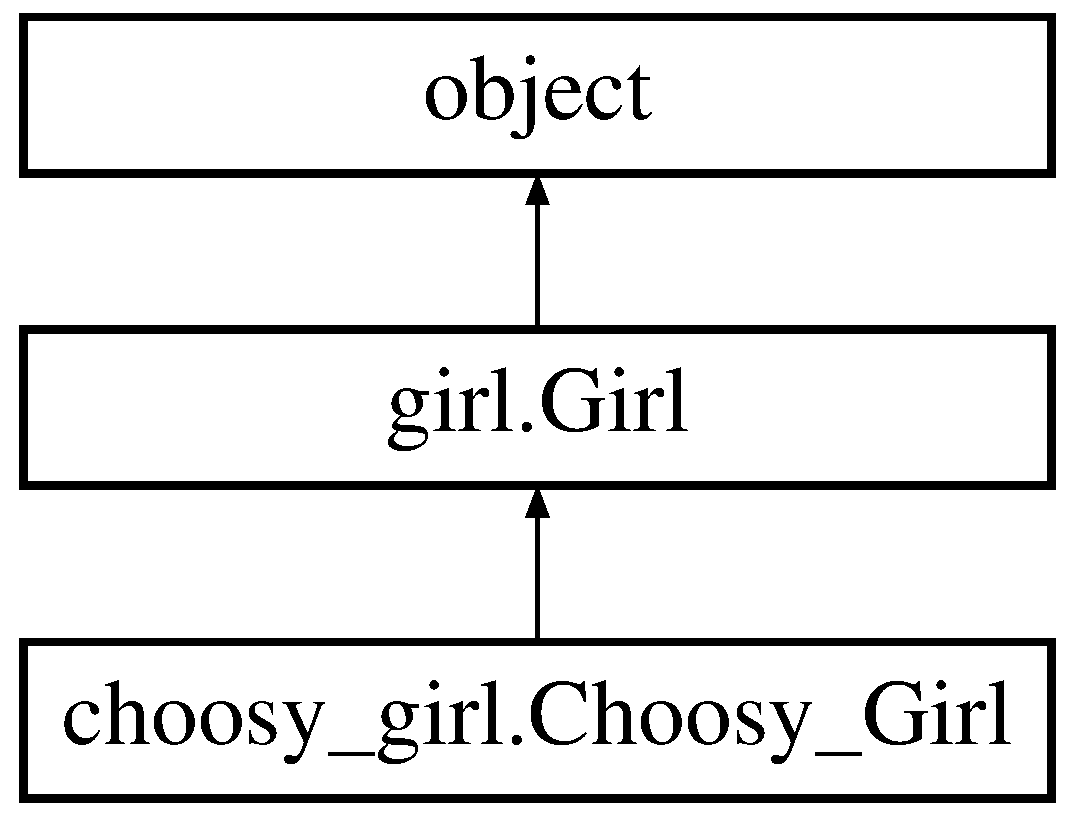
\includegraphics[height=3.000000cm]{classchoosy__girl_1_1_choosy___girl}
\end{center}
\end{figure}
\subsection*{Public Member Functions}
\begin{DoxyCompactItemize}
\item 
\mbox{\Hypertarget{classchoosy__girl_1_1_choosy___girl_af359f24e40dd32cd42b4e556957c4398}\label{classchoosy__girl_1_1_choosy___girl_af359f24e40dd32cd42b4e556957c4398}} 
def {\bfseries \+\_\+\+\_\+init\+\_\+\+\_\+} (self, name, attractiveness, intelligence, maintenance, committed, paired\+\_\+to)
\item 
\mbox{\Hypertarget{classchoosy__girl_1_1_choosy___girl_a0ca3f882f7db874f3d9a8910e1200610}\label{classchoosy__girl_1_1_choosy___girl_a0ca3f882f7db874f3d9a8910e1200610}} 
def {\bfseries giftworth} (self, gift)
\item 
\mbox{\Hypertarget{classchoosy__girl_1_1_choosy___girl_a02611ddf51ba90e2d483ba3895258b5d}\label{classchoosy__girl_1_1_choosy___girl_a02611ddf51ba90e2d483ba3895258b5d}} 
def {\bfseries happiness} (self)
\end{DoxyCompactItemize}
\subsection*{Public Attributes}
\begin{DoxyCompactItemize}
\item 
\mbox{\Hypertarget{classchoosy__girl_1_1_choosy___girl_aa1ed305e2c8a9cec5b7c803dbac497af}\label{classchoosy__girl_1_1_choosy___girl_aa1ed305e2c8a9cec5b7c803dbac497af}} 
{\bfseries type}
\item 
\mbox{\Hypertarget{classchoosy__girl_1_1_choosy___girl_ae997ec53e67e4529d3dba9f3d57fd523}\label{classchoosy__girl_1_1_choosy___girl_ae997ec53e67e4529d3dba9f3d57fd523}} 
{\bfseries gift\+\_\+appreciation}
\end{DoxyCompactItemize}


\subsection{Detailed Description}
\begin{DoxyVerb}Values luxury gifts more.
Luxury gift assigned twice the value.

Happiness is logarithmic function of attribute gift_appreciation
The choosy, whose happiness in a relationship is logarithmic of the total cost of gifts achieved over maintenance. However the luxury gifts are very previous and count double the normal value.\end{DoxyVerb}
 

The documentation for this class was generated from the following file\+:\begin{DoxyCompactItemize}
\item 
choosy\+\_\+girl.\+py\end{DoxyCompactItemize}

\hypertarget{classcouple_1_1_couple}{}\section{couple.\+Couple Class Reference}
\label{classcouple_1_1_couple}\index{couple.\+Couple@{couple.\+Couple}}
Inheritance diagram for couple.\+Couple\+:\begin{figure}[H]
\begin{center}
\leavevmode
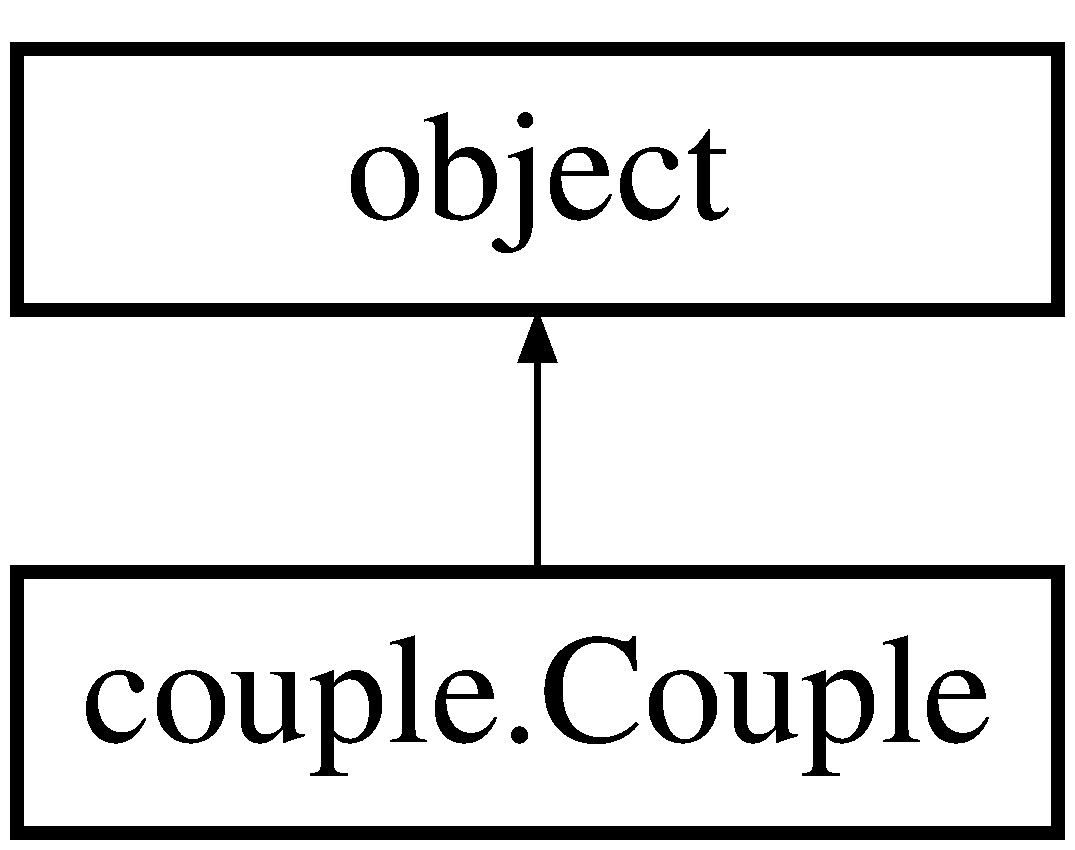
\includegraphics[height=2.000000cm]{classcouple_1_1_couple}
\end{center}
\end{figure}
\subsection*{Public Member Functions}
\begin{DoxyCompactItemize}
\item 
\mbox{\Hypertarget{classcouple_1_1_couple_a3cd6b67c48b545c1b51a8c11ac70677c}\label{classcouple_1_1_couple_a3cd6b67c48b545c1b51a8c11ac70677c}} 
def {\bfseries \+\_\+\+\_\+init\+\_\+\+\_\+} (self, boy, girl)
\item 
def \hyperlink{classcouple_1_1_couple_ab7ac98ab6a0dd03bf75790f949cb0c90}{happiness} (self)
\item 
def \hyperlink{classcouple_1_1_couple_a1752d35bbc3da6524676374511693988}{compatibility} (self)
\end{DoxyCompactItemize}
\subsection*{Public Attributes}
\begin{DoxyCompactItemize}
\item 
\mbox{\Hypertarget{classcouple_1_1_couple_a9add8e4c50bcbf4424339df43ed77df6}\label{classcouple_1_1_couple_a9add8e4c50bcbf4424339df43ed77df6}} 
{\bfseries boy}
\item 
\mbox{\Hypertarget{classcouple_1_1_couple_a99b4aa0aa5cd56aab0edebbba13e31b3}\label{classcouple_1_1_couple_a99b4aa0aa5cd56aab0edebbba13e31b3}} 
{\bfseries girl}
\end{DoxyCompactItemize}


\subsection{Detailed Description}
\begin{DoxyVerb}Has methods  happiness and compatibility
\end{DoxyVerb}
 

\subsection{Member Function Documentation}
\mbox{\Hypertarget{classcouple_1_1_couple_a1752d35bbc3da6524676374511693988}\label{classcouple_1_1_couple_a1752d35bbc3da6524676374511693988}} 
\index{couple\+::\+Couple@{couple\+::\+Couple}!compatibility@{compatibility}}
\index{compatibility@{compatibility}!couple\+::\+Couple@{couple\+::\+Couple}}
\subsubsection{\texorpdfstring{compatibility()}{compatibility()}}
{\footnotesize\ttfamily def couple.\+Couple.\+compatibility (\begin{DoxyParamCaption}\item[{}]{self }\end{DoxyParamCaption})}

\begin{DoxyVerb}The compatibility of a couple is defined as the sum of: magnitude by which the budget of the boy exceeds the maintenance cost of the girl, the absolute value of the difference in attractiveness, and the absolute value of the difference of intelligence.\end{DoxyVerb}
 \mbox{\Hypertarget{classcouple_1_1_couple_ab7ac98ab6a0dd03bf75790f949cb0c90}\label{classcouple_1_1_couple_ab7ac98ab6a0dd03bf75790f949cb0c90}} 
\index{couple\+::\+Couple@{couple\+::\+Couple}!happiness@{happiness}}
\index{happiness@{happiness}!couple\+::\+Couple@{couple\+::\+Couple}}
\subsubsection{\texorpdfstring{happiness()}{happiness()}}
{\footnotesize\ttfamily def couple.\+Couple.\+happiness (\begin{DoxyParamCaption}\item[{}]{self }\end{DoxyParamCaption})}

\begin{DoxyVerb}The happiness of a couple is defined as the sum of the happiness of both girl and boy.
\end{DoxyVerb}
 

The documentation for this class was generated from the following file\+:\begin{DoxyCompactItemize}
\item 
/\+Users/invokesus/assignment/couple.\+py\end{DoxyCompactItemize}

\hypertarget{classdesperate__girl_1_1_desperate___girl}{}\section{desperate\+\_\+girl.\+Desperate\+\_\+\+Girl Class Reference}
\label{classdesperate__girl_1_1_desperate___girl}\index{desperate\+\_\+girl.\+Desperate\+\_\+\+Girl@{desperate\+\_\+girl.\+Desperate\+\_\+\+Girl}}
\subsection*{Public Member Functions}
\begin{DoxyCompactItemize}
\item 
\mbox{\Hypertarget{classdesperate__girl_1_1_desperate___girl_ab79e28f51333e510187e105106ec8dca}\label{classdesperate__girl_1_1_desperate___girl_ab79e28f51333e510187e105106ec8dca}} 
def {\bfseries \+\_\+\+\_\+init\+\_\+\+\_\+} (self, name, attractiveness, intelligence, maintenance, committed, paired\+\_\+to)
\item 
\mbox{\Hypertarget{classdesperate__girl_1_1_desperate___girl_ad840fc289e5dc74f86133a429f3b145d}\label{classdesperate__girl_1_1_desperate___girl_ad840fc289e5dc74f86133a429f3b145d}} 
def {\bfseries giftworth} (self, gift)
\item 
\mbox{\Hypertarget{classdesperate__girl_1_1_desperate___girl_af80bc07443149f82a9d17d2f86a0c06a}\label{classdesperate__girl_1_1_desperate___girl_af80bc07443149f82a9d17d2f86a0c06a}} 
def {\bfseries happiness} (self)
\end{DoxyCompactItemize}
\subsection*{Public Attributes}
\begin{DoxyCompactItemize}
\item 
\mbox{\Hypertarget{classdesperate__girl_1_1_desperate___girl_a09f294c963c5b67278861e6ca00c7f6d}\label{classdesperate__girl_1_1_desperate___girl_a09f294c963c5b67278861e6ca00c7f6d}} 
{\bfseries name}
\item 
\mbox{\Hypertarget{classdesperate__girl_1_1_desperate___girl_affeed709b0bdb8c8c7250fe7ee5c77b4}\label{classdesperate__girl_1_1_desperate___girl_affeed709b0bdb8c8c7250fe7ee5c77b4}} 
{\bfseries attractiveness}
\item 
\mbox{\Hypertarget{classdesperate__girl_1_1_desperate___girl_a7c861186b97d1e17d1290813baa836c2}\label{classdesperate__girl_1_1_desperate___girl_a7c861186b97d1e17d1290813baa836c2}} 
{\bfseries intelligence}
\item 
\mbox{\Hypertarget{classdesperate__girl_1_1_desperate___girl_a0737a668754634c2706e6a01b442670e}\label{classdesperate__girl_1_1_desperate___girl_a0737a668754634c2706e6a01b442670e}} 
{\bfseries maintenance}
\item 
\mbox{\Hypertarget{classdesperate__girl_1_1_desperate___girl_a3afc3b57cd5fdbbf47487772047c0f70}\label{classdesperate__girl_1_1_desperate___girl_a3afc3b57cd5fdbbf47487772047c0f70}} 
{\bfseries committed}
\item 
\mbox{\Hypertarget{classdesperate__girl_1_1_desperate___girl_ab94bc99816a300146110fd6cfb3823c3}\label{classdesperate__girl_1_1_desperate___girl_ab94bc99816a300146110fd6cfb3823c3}} 
{\bfseries paired\+\_\+to}
\item 
\mbox{\Hypertarget{classdesperate__girl_1_1_desperate___girl_a55e8038abc86bd1a207878a70dac24c7}\label{classdesperate__girl_1_1_desperate___girl_a55e8038abc86bd1a207878a70dac24c7}} 
{\bfseries type}
\item 
\mbox{\Hypertarget{classdesperate__girl_1_1_desperate___girl_ac177c9aef939da3b0830fccfda51eb51}\label{classdesperate__girl_1_1_desperate___girl_ac177c9aef939da3b0830fccfda51eb51}} 
{\bfseries gift\+\_\+appreciation}
\end{DoxyCompactItemize}


\subsection{Detailed Description}
\begin{DoxyVerb}Happiness is exponential function of attribute gift_appreciation
The desperate, whose happiness in a relationship is exponential to the total cost of gifts received over maintenance, including luxury gifts. The value is not considered.
\end{DoxyVerb}
 

The documentation for this class was generated from the following file\+:\begin{DoxyCompactItemize}
\item 
/\+Users/invokesus/assignment/desperate\+\_\+girl.\+py\end{DoxyCompactItemize}

\hypertarget{classessential__gift_1_1_essential___gift}{}\section{essential\+\_\+gift.\+Essential\+\_\+\+Gift Class Reference}
\label{classessential__gift_1_1_essential___gift}\index{essential\+\_\+gift.\+Essential\+\_\+\+Gift@{essential\+\_\+gift.\+Essential\+\_\+\+Gift}}
Inheritance diagram for essential\+\_\+gift.\+Essential\+\_\+\+Gift\+:\begin{figure}[H]
\begin{center}
\leavevmode
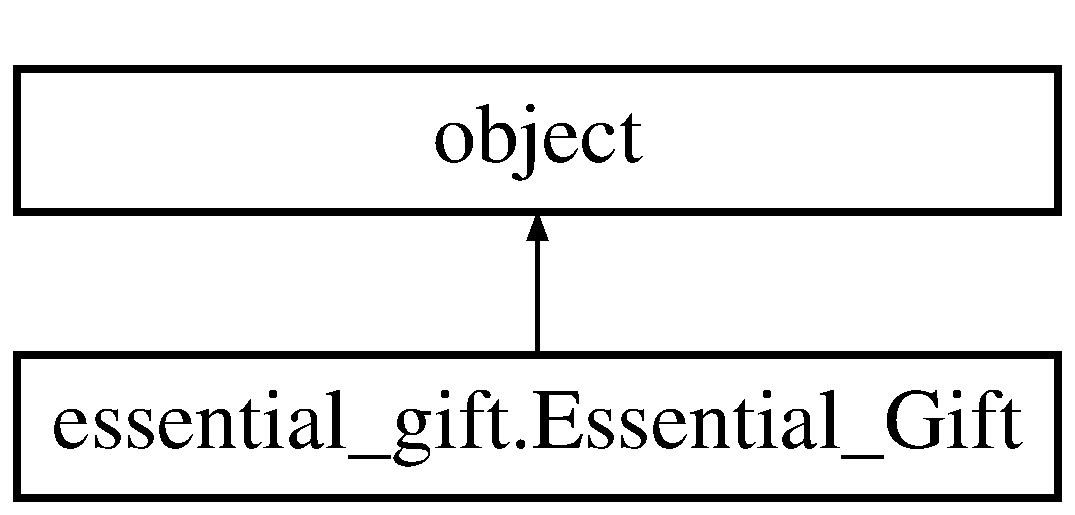
\includegraphics[height=2.000000cm]{classessential__gift_1_1_essential___gift}
\end{center}
\end{figure}
\subsection*{Public Member Functions}
\begin{DoxyCompactItemize}
\item 
\mbox{\Hypertarget{classessential__gift_1_1_essential___gift_a3425b38913d6abbb0d2976ea3339aadd}\label{classessential__gift_1_1_essential___gift_a3425b38913d6abbb0d2976ea3339aadd}} 
def {\bfseries \+\_\+\+\_\+init\+\_\+\+\_\+} (self, price, value)
\end{DoxyCompactItemize}
\subsection*{Public Attributes}
\begin{DoxyCompactItemize}
\item 
\mbox{\Hypertarget{classessential__gift_1_1_essential___gift_aa0895da6a47b0591270e45f564f31fe4}\label{classessential__gift_1_1_essential___gift_aa0895da6a47b0591270e45f564f31fe4}} 
{\bfseries price}
\item 
\mbox{\Hypertarget{classessential__gift_1_1_essential___gift_a0efdc8693deea51040a398e296bfece7}\label{classessential__gift_1_1_essential___gift_a0efdc8693deea51040a398e296bfece7}} 
{\bfseries value}
\end{DoxyCompactItemize}


\subsection{Detailed Description}
\begin{DoxyVerb}Bare minimal gifts and are associated with a price and value.
\end{DoxyVerb}
 

The documentation for this class was generated from the following file\+:\begin{DoxyCompactItemize}
\item 
/\+Users/invokesus/assignment/essential\+\_\+gift.\+py\end{DoxyCompactItemize}

\hypertarget{classgeek__boy_1_1_geek___boy}{}\section{geek\+\_\+boy.\+Geek\+\_\+\+Boy Class Reference}
\label{classgeek__boy_1_1_geek___boy}\index{geek\+\_\+boy.\+Geek\+\_\+\+Boy@{geek\+\_\+boy.\+Geek\+\_\+\+Boy}}
Inheritance diagram for geek\+\_\+boy.\+Geek\+\_\+\+Boy\+:\begin{figure}[H]
\begin{center}
\leavevmode
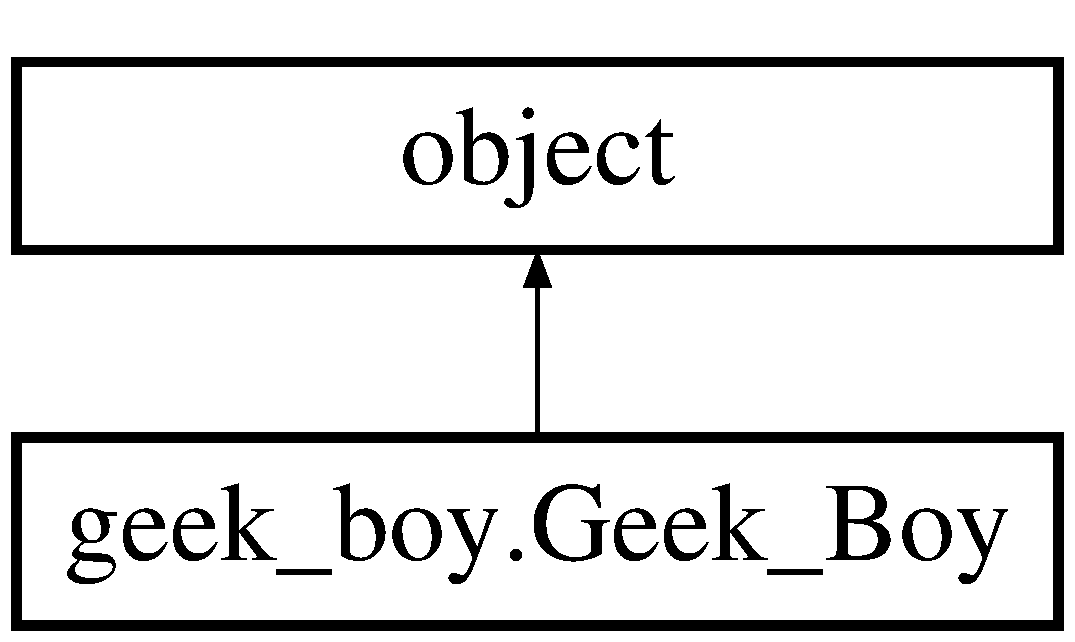
\includegraphics[height=2.000000cm]{classgeek__boy_1_1_geek___boy}
\end{center}
\end{figure}
\subsection*{Public Member Functions}
\begin{DoxyCompactItemize}
\item 
\mbox{\Hypertarget{classgeek__boy_1_1_geek___boy_ae4df402c3dda6877a3957e4bdd41b228}\label{classgeek__boy_1_1_geek___boy_ae4df402c3dda6877a3957e4bdd41b228}} 
def {\bfseries \+\_\+\+\_\+init\+\_\+\+\_\+} (self, name, attractiveness, intelligence, budget, attraction\+\_\+requirement, committed, expenditure, paired\+\_\+to)
\item 
\mbox{\Hypertarget{classgeek__boy_1_1_geek___boy_a651f4b0e255c1585737ffd0a93099edd}\label{classgeek__boy_1_1_geek___boy_a651f4b0e255c1585737ffd0a93099edd}} 
def {\bfseries happiness} (self, g)
\end{DoxyCompactItemize}
\subsection*{Public Attributes}
\begin{DoxyCompactItemize}
\item 
\mbox{\Hypertarget{classgeek__boy_1_1_geek___boy_a6c9ca7bc6b462250e768550a672db759}\label{classgeek__boy_1_1_geek___boy_a6c9ca7bc6b462250e768550a672db759}} 
{\bfseries name}
\item 
\mbox{\Hypertarget{classgeek__boy_1_1_geek___boy_a03843bf99e532745dfcfcda585779110}\label{classgeek__boy_1_1_geek___boy_a03843bf99e532745dfcfcda585779110}} 
{\bfseries attractiveness}
\item 
\mbox{\Hypertarget{classgeek__boy_1_1_geek___boy_a2c8a57c6e3b35b904b992aa764cbf759}\label{classgeek__boy_1_1_geek___boy_a2c8a57c6e3b35b904b992aa764cbf759}} 
{\bfseries intelligence}
\item 
\mbox{\Hypertarget{classgeek__boy_1_1_geek___boy_aafd75f742227ec6ca3911091671e888d}\label{classgeek__boy_1_1_geek___boy_aafd75f742227ec6ca3911091671e888d}} 
{\bfseries budget}
\item 
\mbox{\Hypertarget{classgeek__boy_1_1_geek___boy_af14e4f6d5e00e4f27ac60ba68a28af33}\label{classgeek__boy_1_1_geek___boy_af14e4f6d5e00e4f27ac60ba68a28af33}} 
{\bfseries attraction\+\_\+requirement}
\item 
\mbox{\Hypertarget{classgeek__boy_1_1_geek___boy_aab19a0ea9c20343ef7d3a1e0d209c7fa}\label{classgeek__boy_1_1_geek___boy_aab19a0ea9c20343ef7d3a1e0d209c7fa}} 
{\bfseries committed}
\item 
\mbox{\Hypertarget{classgeek__boy_1_1_geek___boy_a32e7bd57e5ed1595bd47d67a0fd40029}\label{classgeek__boy_1_1_geek___boy_a32e7bd57e5ed1595bd47d67a0fd40029}} 
{\bfseries expenditure}
\item 
\mbox{\Hypertarget{classgeek__boy_1_1_geek___boy_a254e9ad875c879c22b8c45ed8a3dd601}\label{classgeek__boy_1_1_geek___boy_a254e9ad875c879c22b8c45ed8a3dd601}} 
{\bfseries paired\+\_\+to}
\item 
\mbox{\Hypertarget{classgeek__boy_1_1_geek___boy_a835570f9058c1e3326de0dd3d699de99}\label{classgeek__boy_1_1_geek___boy_a835570f9058c1e3326de0dd3d699de99}} 
{\bfseries happiness}
\item 
\mbox{\Hypertarget{classgeek__boy_1_1_geek___boy_a3331fb6dfe37cf9913ab14b36b4aa205}\label{classgeek__boy_1_1_geek___boy_a3331fb6dfe37cf9913ab14b36b4aa205}} 
{\bfseries type}
\end{DoxyCompactItemize}


The documentation for this class was generated from the following file\+:\begin{DoxyCompactItemize}
\item 
/\+Users/invokesus/assignment/geek\+\_\+boy.\+py\end{DoxyCompactItemize}

\hypertarget{classgenerous__boy_1_1_generous___boy}{}\section{generous\+\_\+boy.\+Generous\+\_\+\+Boy Class Reference}
\label{classgenerous__boy_1_1_generous___boy}\index{generous\+\_\+boy.\+Generous\+\_\+\+Boy@{generous\+\_\+boy.\+Generous\+\_\+\+Boy}}
\subsection*{Public Member Functions}
\begin{DoxyCompactItemize}
\item 
\mbox{\Hypertarget{classgenerous__boy_1_1_generous___boy_a0b255a2a43d52138254fb384eeb8ca4b}\label{classgenerous__boy_1_1_generous___boy_a0b255a2a43d52138254fb384eeb8ca4b}} 
def {\bfseries \+\_\+\+\_\+init\+\_\+\+\_\+} (self, name, attractiveness, intelligence, budget, attraction\+\_\+requirement, committed, expenditure, paired\+\_\+to)
\item 
\mbox{\Hypertarget{classgenerous__boy_1_1_generous___boy_a0fe95bfe65726fcffdf859b0ae03932f}\label{classgenerous__boy_1_1_generous___boy_a0fe95bfe65726fcffdf859b0ae03932f}} 
def {\bfseries happiness} (self, g)
\end{DoxyCompactItemize}
\subsection*{Public Attributes}
\begin{DoxyCompactItemize}
\item 
\mbox{\Hypertarget{classgenerous__boy_1_1_generous___boy_afd3c6e06f846ba4296d01295d72a2761}\label{classgenerous__boy_1_1_generous___boy_afd3c6e06f846ba4296d01295d72a2761}} 
{\bfseries name}
\item 
\mbox{\Hypertarget{classgenerous__boy_1_1_generous___boy_a21fd9c49689d0def38d62a5f3bc267eb}\label{classgenerous__boy_1_1_generous___boy_a21fd9c49689d0def38d62a5f3bc267eb}} 
{\bfseries attractiveness}
\item 
\mbox{\Hypertarget{classgenerous__boy_1_1_generous___boy_a9ca95d569e31ac9f1fafc8c98c0d24ff}\label{classgenerous__boy_1_1_generous___boy_a9ca95d569e31ac9f1fafc8c98c0d24ff}} 
{\bfseries intelligence}
\item 
\mbox{\Hypertarget{classgenerous__boy_1_1_generous___boy_aacff3eee77e181ca4e813b8d3739db4f}\label{classgenerous__boy_1_1_generous___boy_aacff3eee77e181ca4e813b8d3739db4f}} 
{\bfseries budget}
\item 
\mbox{\Hypertarget{classgenerous__boy_1_1_generous___boy_a4042ce73df5df4644d0468d19ef9b4ef}\label{classgenerous__boy_1_1_generous___boy_a4042ce73df5df4644d0468d19ef9b4ef}} 
{\bfseries attraction\+\_\+requirement}
\item 
\mbox{\Hypertarget{classgenerous__boy_1_1_generous___boy_a3093f9f591a9fbcae8209df25d73817a}\label{classgenerous__boy_1_1_generous___boy_a3093f9f591a9fbcae8209df25d73817a}} 
{\bfseries committed}
\item 
\mbox{\Hypertarget{classgenerous__boy_1_1_generous___boy_a9e51187bb8da4d5a31b94e568a00f745}\label{classgenerous__boy_1_1_generous___boy_a9e51187bb8da4d5a31b94e568a00f745}} 
{\bfseries expenditure}
\item 
\mbox{\Hypertarget{classgenerous__boy_1_1_generous___boy_a88dc19afb1baaa99e8256f3f7d40309c}\label{classgenerous__boy_1_1_generous___boy_a88dc19afb1baaa99e8256f3f7d40309c}} 
{\bfseries paired\+\_\+to}
\item 
\mbox{\Hypertarget{classgenerous__boy_1_1_generous___boy_a7461b9bcdb7f0531e3cd9ba2b48aa535}\label{classgenerous__boy_1_1_generous___boy_a7461b9bcdb7f0531e3cd9ba2b48aa535}} 
{\bfseries happiness}
\item 
\mbox{\Hypertarget{classgenerous__boy_1_1_generous___boy_a23cec95ad272bb25b7b3be28e07fff43}\label{classgenerous__boy_1_1_generous___boy_a23cec95ad272bb25b7b3be28e07fff43}} 
{\bfseries type}
\end{DoxyCompactItemize}


The documentation for this class was generated from the following file\+:\begin{DoxyCompactItemize}
\item 
/\+Users/invokesus/assignment/generous\+\_\+boy.\+py\end{DoxyCompactItemize}

\hypertarget{classluxury__gift_1_1_luxury___gift}{}\section{luxury\+\_\+gift.\+Luxury\+\_\+\+Gift Class Reference}
\label{classluxury__gift_1_1_luxury___gift}\index{luxury\+\_\+gift.\+Luxury\+\_\+\+Gift@{luxury\+\_\+gift.\+Luxury\+\_\+\+Gift}}
Inheritance diagram for luxury\+\_\+gift.\+Luxury\+\_\+\+Gift\+:\begin{figure}[H]
\begin{center}
\leavevmode
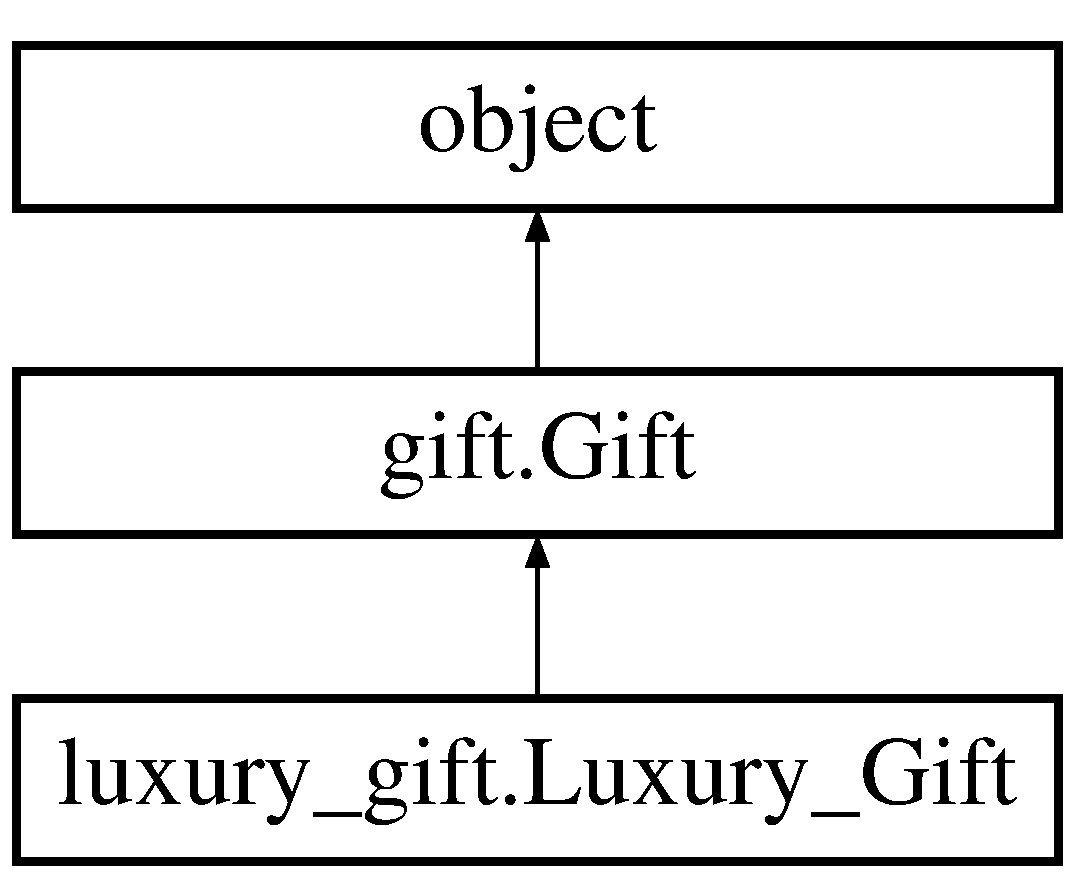
\includegraphics[height=3.000000cm]{classluxury__gift_1_1_luxury___gift}
\end{center}
\end{figure}
\subsection*{Public Member Functions}
\begin{DoxyCompactItemize}
\item 
\mbox{\Hypertarget{classluxury__gift_1_1_luxury___gift_ab93b10ec0683264d2c821a4963dd1dd2}\label{classluxury__gift_1_1_luxury___gift_ab93b10ec0683264d2c821a4963dd1dd2}} 
def {\bfseries \+\_\+\+\_\+init\+\_\+\+\_\+} (self, price, value, luxury\+\_\+rating, difficulty\+\_\+to\+\_\+obtain)
\end{DoxyCompactItemize}
\subsection*{Public Attributes}
\begin{DoxyCompactItemize}
\item 
\mbox{\Hypertarget{classluxury__gift_1_1_luxury___gift_a6663d4dd880f62c54414f404de3c6643}\label{classluxury__gift_1_1_luxury___gift_a6663d4dd880f62c54414f404de3c6643}} 
{\bfseries luxury\+\_\+rating}
\item 
\mbox{\Hypertarget{classluxury__gift_1_1_luxury___gift_a585dc4d044e9bac12b7691aa8fd56076}\label{classluxury__gift_1_1_luxury___gift_a585dc4d044e9bac12b7691aa8fd56076}} 
{\bfseries difficulty\+\_\+to\+\_\+obtain}
\end{DoxyCompactItemize}


\subsection{Detailed Description}
\begin{DoxyVerb}Attributes of the luxury rating, difficulty to obtain the gift, value and price.
\end{DoxyVerb}
 

The documentation for this class was generated from the following file\+:\begin{DoxyCompactItemize}
\item 
luxury\+\_\+gift.\+py\end{DoxyCompactItemize}

\hypertarget{classmiser__boy_1_1_miser___boy}{}\section{miser\+\_\+boy.\+Miser\+\_\+\+Boy Class Reference}
\label{classmiser__boy_1_1_miser___boy}\index{miser\+\_\+boy.\+Miser\+\_\+\+Boy@{miser\+\_\+boy.\+Miser\+\_\+\+Boy}}
Inheritance diagram for miser\+\_\+boy.\+Miser\+\_\+\+Boy\+:\begin{figure}[H]
\begin{center}
\leavevmode
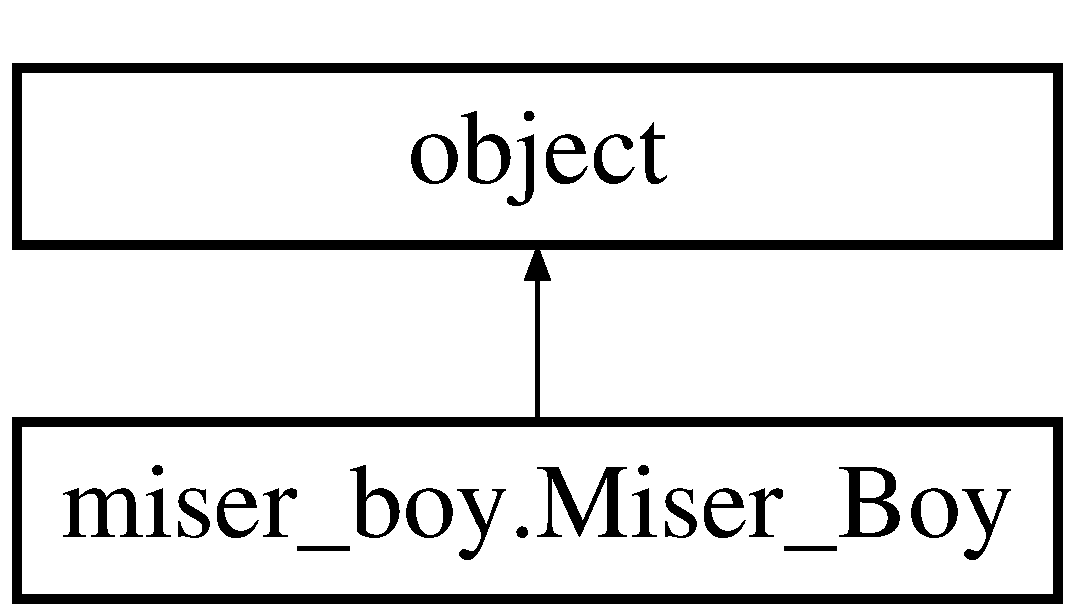
\includegraphics[height=3.000000cm]{classmiser__boy_1_1_miser___boy}
\end{center}
\end{figure}
\subsection*{Public Member Functions}
\begin{DoxyCompactItemize}
\item 
\mbox{\Hypertarget{classmiser__boy_1_1_miser___boy_a5d920fd6f24fcf5c7308e4f8e785c174}\label{classmiser__boy_1_1_miser___boy_a5d920fd6f24fcf5c7308e4f8e785c174}} 
def {\bfseries \+\_\+\+\_\+init\+\_\+\+\_\+} (self, name, attractiveness, intelligence, budget, attraction\+\_\+requirement, committed, expenditure, paired\+\_\+to)
\item 
\mbox{\Hypertarget{classmiser__boy_1_1_miser___boy_a796e7ead0e4d390d3d27aa8ef6802840}\label{classmiser__boy_1_1_miser___boy_a796e7ead0e4d390d3d27aa8ef6802840}} 
def {\bfseries happiness} (self, args)
\end{DoxyCompactItemize}
\subsection*{Public Attributes}
\begin{DoxyCompactItemize}
\item 
\mbox{\Hypertarget{classmiser__boy_1_1_miser___boy_a2380dbb7e2289a7556b8bc9eb1e24466}\label{classmiser__boy_1_1_miser___boy_a2380dbb7e2289a7556b8bc9eb1e24466}} 
{\bfseries type}
\item 
\mbox{\Hypertarget{classmiser__boy_1_1_miser___boy_acb776c80b3541f1efe5f66c81a8c4524}\label{classmiser__boy_1_1_miser___boy_acb776c80b3541f1efe5f66c81a8c4524}} 
{\bfseries happiness}
\end{DoxyCompactItemize}


The documentation for this class was generated from the following file\+:\begin{DoxyCompactItemize}
\item 
miser\+\_\+boy.\+py\end{DoxyCompactItemize}

\hypertarget{classnormal__girl_1_1_normal___girl}{}\section{normal\+\_\+girl.\+Normal\+\_\+\+Girl Class Reference}
\label{classnormal__girl_1_1_normal___girl}\index{normal\+\_\+girl.\+Normal\+\_\+\+Girl@{normal\+\_\+girl.\+Normal\+\_\+\+Girl}}
Inheritance diagram for normal\+\_\+girl.\+Normal\+\_\+\+Girl\+:\begin{figure}[H]
\begin{center}
\leavevmode
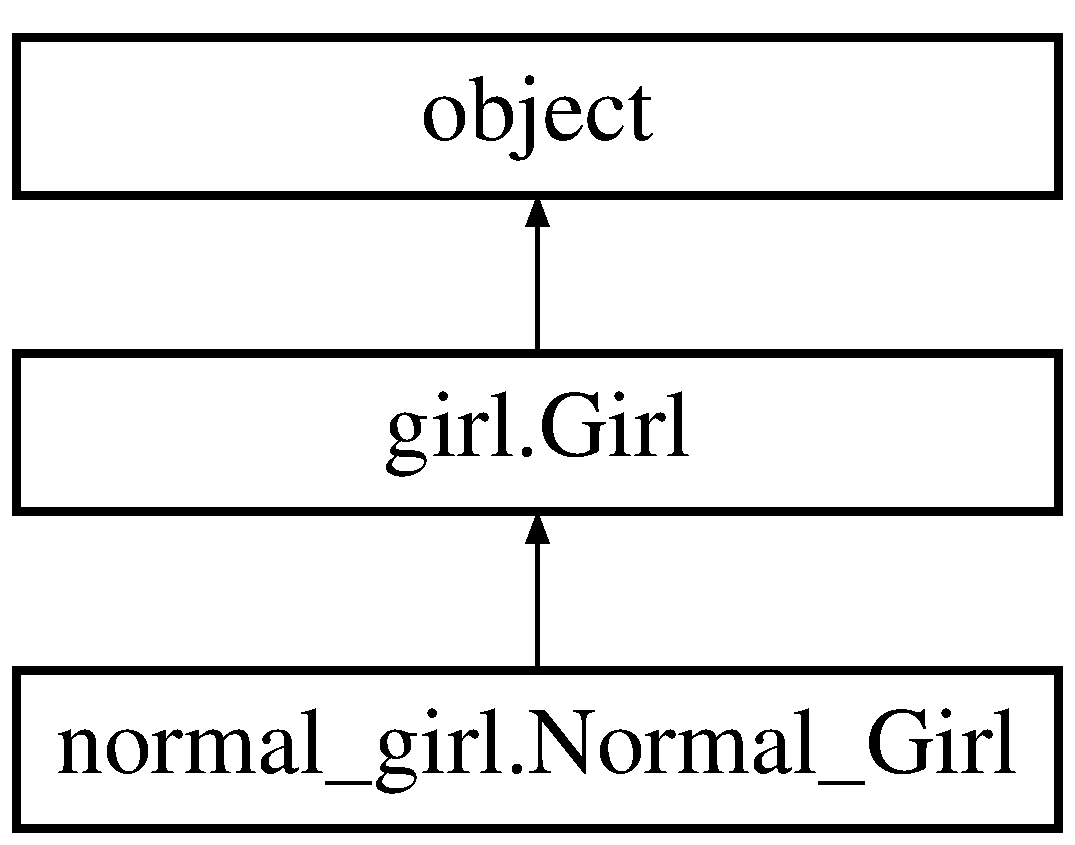
\includegraphics[height=2.000000cm]{classnormal__girl_1_1_normal___girl}
\end{center}
\end{figure}
\subsection*{Public Member Functions}
\begin{DoxyCompactItemize}
\item 
\mbox{\Hypertarget{classnormal__girl_1_1_normal___girl_a8fc16ab0acaf0997b8a4c5e0c2b57a0c}\label{classnormal__girl_1_1_normal___girl_a8fc16ab0acaf0997b8a4c5e0c2b57a0c}} 
def {\bfseries \+\_\+\+\_\+init\+\_\+\+\_\+} (self, name, attractiveness, intelligence, maintenance, committed, paired\+\_\+to)
\item 
\mbox{\Hypertarget{classnormal__girl_1_1_normal___girl_ae7d0d26c0cfbf8152fba9113ff9ef763}\label{classnormal__girl_1_1_normal___girl_ae7d0d26c0cfbf8152fba9113ff9ef763}} 
def {\bfseries giftworth} (self, gift)
\item 
\mbox{\Hypertarget{classnormal__girl_1_1_normal___girl_a6508d58dab5d0c59d769f3f0c1325b46}\label{classnormal__girl_1_1_normal___girl_a6508d58dab5d0c59d769f3f0c1325b46}} 
def {\bfseries happiness} (self)
\end{DoxyCompactItemize}
\subsection*{Public Attributes}
\begin{DoxyCompactItemize}
\item 
\mbox{\Hypertarget{classnormal__girl_1_1_normal___girl_ac6ce282217638dbd0e18294e8fd6ea87}\label{classnormal__girl_1_1_normal___girl_ac6ce282217638dbd0e18294e8fd6ea87}} 
{\bfseries name}
\item 
\mbox{\Hypertarget{classnormal__girl_1_1_normal___girl_a8124c0797d5bf37f820de629367a5ee6}\label{classnormal__girl_1_1_normal___girl_a8124c0797d5bf37f820de629367a5ee6}} 
{\bfseries attractiveness}
\item 
\mbox{\Hypertarget{classnormal__girl_1_1_normal___girl_a6e13ef914384e8b71ab9b1322d9a8674}\label{classnormal__girl_1_1_normal___girl_a6e13ef914384e8b71ab9b1322d9a8674}} 
{\bfseries intelligence}
\item 
\mbox{\Hypertarget{classnormal__girl_1_1_normal___girl_a1807ad41310412d615a5b9929132b181}\label{classnormal__girl_1_1_normal___girl_a1807ad41310412d615a5b9929132b181}} 
{\bfseries maintenance}
\item 
\mbox{\Hypertarget{classnormal__girl_1_1_normal___girl_a5323e9a7a3dbe63723110d47cb975596}\label{classnormal__girl_1_1_normal___girl_a5323e9a7a3dbe63723110d47cb975596}} 
{\bfseries committed}
\item 
\mbox{\Hypertarget{classnormal__girl_1_1_normal___girl_a7fa753a9edfb1e92e23b5c664d08552b}\label{classnormal__girl_1_1_normal___girl_a7fa753a9edfb1e92e23b5c664d08552b}} 
{\bfseries paired\+\_\+to}
\item 
\mbox{\Hypertarget{classnormal__girl_1_1_normal___girl_a43fad908acb615885991aa3f76a3a8b4}\label{classnormal__girl_1_1_normal___girl_a43fad908acb615885991aa3f76a3a8b4}} 
{\bfseries gift\+\_\+appreciation}
\item 
\mbox{\Hypertarget{classnormal__girl_1_1_normal___girl_a2b09c350fa195f1532cff9689276e0a2}\label{classnormal__girl_1_1_normal___girl_a2b09c350fa195f1532cff9689276e0a2}} 
{\bfseries type}
\end{DoxyCompactItemize}


\subsection{Detailed Description}
\begin{DoxyVerb}The choosy, whose happiness in a relationship is logarithmic of the total cost of gifts achieved over maintenance. However the luxury gifts are very previous and count double the normal value.
\end{DoxyVerb}
 

The documentation for this class was generated from the following file\+:\begin{DoxyCompactItemize}
\item 
/\+Users/invokesus/assignment/normal\+\_\+girl.\+py\end{DoxyCompactItemize}

\hypertarget{classutility__gift_1_1_utility___gift}{}\section{utility\+\_\+gift.\+Utility\+\_\+\+Gift Class Reference}
\label{classutility__gift_1_1_utility___gift}\index{utility\+\_\+gift.\+Utility\+\_\+\+Gift@{utility\+\_\+gift.\+Utility\+\_\+\+Gift}}
\subsection*{Public Member Functions}
\begin{DoxyCompactItemize}
\item 
\mbox{\Hypertarget{classutility__gift_1_1_utility___gift_aa052e2d051b6ed87c8a1063994c6d625}\label{classutility__gift_1_1_utility___gift_aa052e2d051b6ed87c8a1063994c6d625}} 
def {\bfseries \+\_\+\+\_\+init\+\_\+\+\_\+} (self, price, value, utility\+\_\+value, utility\+\_\+class)
\end{DoxyCompactItemize}
\subsection*{Public Attributes}
\begin{DoxyCompactItemize}
\item 
\mbox{\Hypertarget{classutility__gift_1_1_utility___gift_a07cbe189b2d18ea5be913c1504494876}\label{classutility__gift_1_1_utility___gift_a07cbe189b2d18ea5be913c1504494876}} 
{\bfseries price}
\item 
\mbox{\Hypertarget{classutility__gift_1_1_utility___gift_ad6bfd57dd19981207c362567a99257f1}\label{classutility__gift_1_1_utility___gift_ad6bfd57dd19981207c362567a99257f1}} 
{\bfseries value}
\item 
\mbox{\Hypertarget{classutility__gift_1_1_utility___gift_a4e6bdcfbda7e752922e9e5a9a5589aeb}\label{classutility__gift_1_1_utility___gift_a4e6bdcfbda7e752922e9e5a9a5589aeb}} 
{\bfseries utility\+\_\+view}
\item 
\mbox{\Hypertarget{classutility__gift_1_1_utility___gift_a7e3112caebf026d3e0c583504e1f5a5c}\label{classutility__gift_1_1_utility___gift_a7e3112caebf026d3e0c583504e1f5a5c}} 
{\bfseries utility\+\_\+class}
\end{DoxyCompactItemize}


\subsection{Detailed Description}
\begin{DoxyVerb}Associated with the utility value, utility class, value and price. 
\end{DoxyVerb}
 

The documentation for this class was generated from the following file\+:\begin{DoxyCompactItemize}
\item 
/\+Users/invokesus/assignment/utility\+\_\+gift.\+py\end{DoxyCompactItemize}

%--- End generated contents ---

% Index
\backmatter
\newpage
\phantomsection
\clearemptydoublepage
\addcontentsline{toc}{chapter}{Index}
\printindex

\end{document}
